\documentclass[UTF8]{ctexart}
\usepackage{geometry}
\geometry{a4paper,centering,scale=0.8}
\usepackage[format=hang,font=small,textfont=it]{caption}
\usepackage[nottoc]{tocbibind}%nottoc表示不包含目录本身
\usepackage{fontenc}
\punctstyle{quanjiao}
\usepackage{graphicx}
\usepackage[numbers,square,compress,merge]{natbib}
\usepackage{gbt7714}
\usepackage{amsmath}


%\usepackage{array}
%\usepackage{booktabs}
\title{\heiti 勾股定理}
\author{张三}
\date{\today}
\newtheorem{thm}{定理}
\bibliographystyle{gbt7714-numerical}
\DeclareMathOperator\dif{d\!}

\newenvironment{myquote}
{\begin{quote}\kaishu\zihao{-5}}
{\end{quote}}

\begin{document}

\maketitle
\tableofcontents
\section{勾股定理在古代}
\label{section:A}
2022年是进入全面建设社会主义现代化国家\footnote{国家}、向第二个百年奋斗目标进军新征程的重要一年,
\begin{thm}[召开大会]
中国共产党将召开第二十次全国人民代表大会,此次大会将为中国之后几年甚至几十年的发展定下基调。
\end{thm}
通过学习二十大精神并了解二十大中做出的决议、政策,我们支部的成员能更好地继续发扬历史主动精神,
为全面建设社会主义现代化国家贡献出我们的\emph{“青春力量”}。
\begin{figure}[ht]%h表示here,t表示top
	\centering
	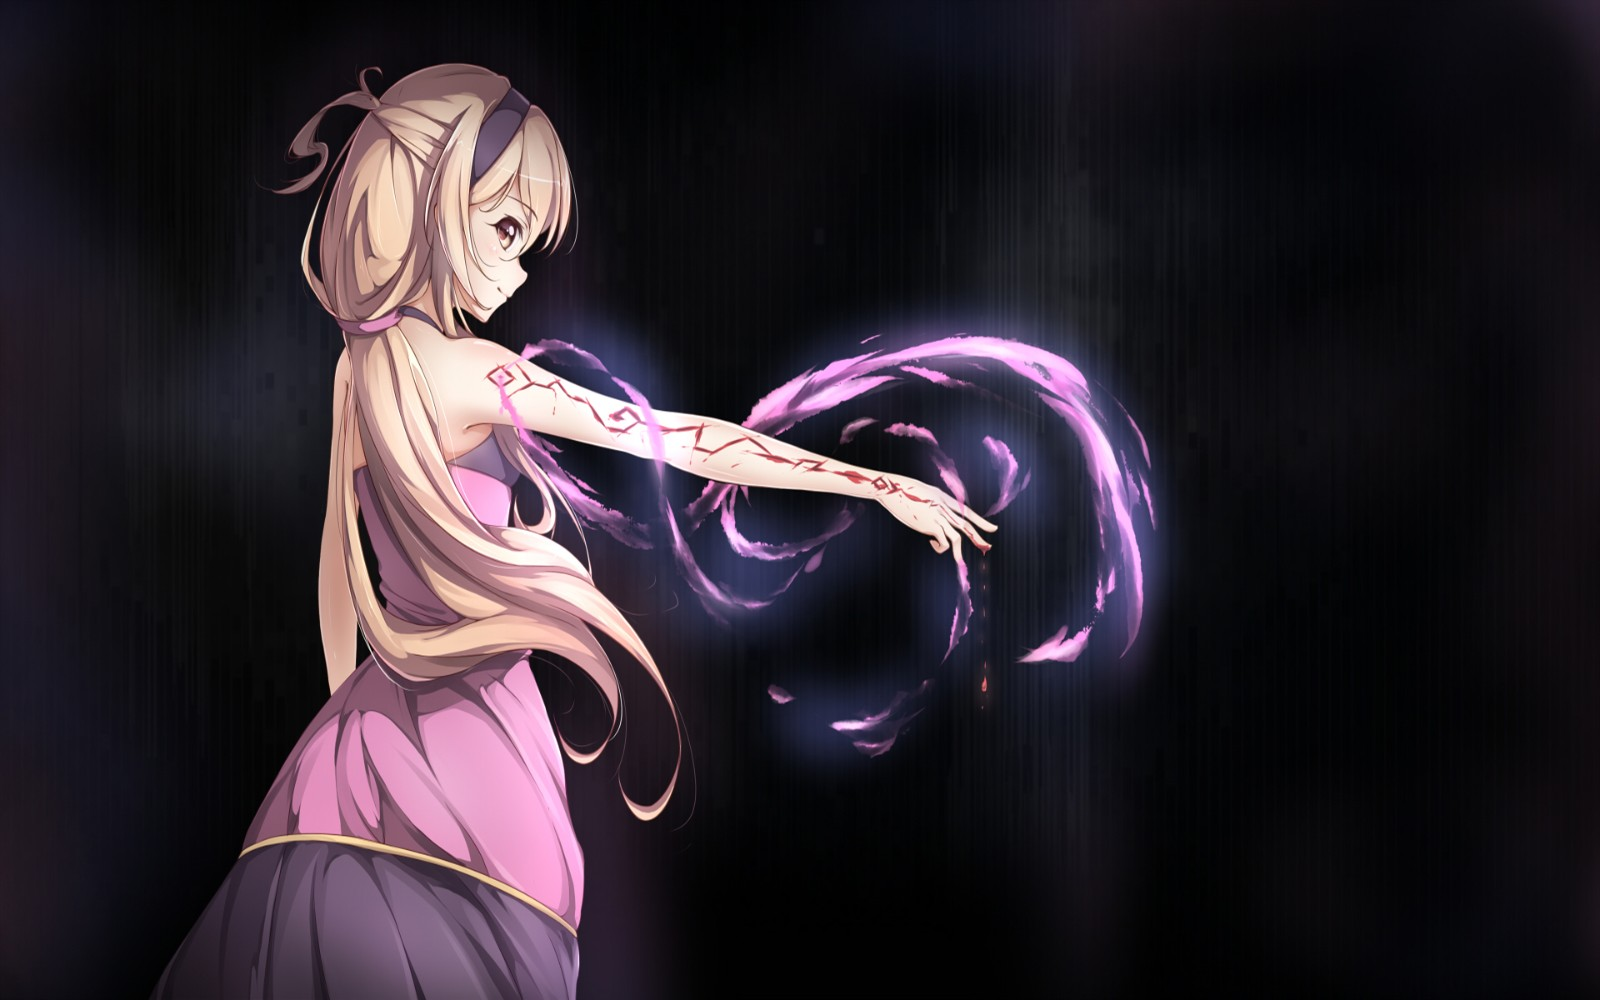
\includegraphics[width=4cm]{2.jpg}
	\caption{这是一个示例图}
	\label{fig:shili}
\end{figure}
\newtheorem{lemma}{引理}[section]
\begin{lemma}
	sdf
\end{lemma}

\begin{lemma}
	sdfjss
\end{lemma}
\newtheorem{prop}[thm]{命题}
\begin{prop}
	kkkkkk
\end{prop}

\begin{thm}
	
	sdfdfsdf
\end{thm}



\section{勾股定理的近代形式}
\begin{table}[h]
	\centering
\begin{tabular}{|rrr|}
	\hline
	直角边$a$ & 直角边$b$ & 斜边$c$\\
	\hline
	3 & 4 & 5\\
	5 &12 &13\\
	\hline
	
\end{tabular}%
\qquad
($a^2 + b^2 = c^2$)
\end{table}
我们将以一次集体观影理论学习活动拉开整个团改金系列活动的序幕,让支部成员先对全国人民代表大会有一些基础的认识,并激发大家深入学习的兴趣。我们将要观看的纪录片是\cite{杨俊林,王建华,魏跃新2020}

\begin{lemma}
	sdfj
\end{lemma}
\begin{myquote}
《光辉历程——纪念全国人民代表大会成立六十周年》
\end{myquote}
	
该片主要介绍了新中国成立后,人民代表会议的成功实践,为人民代表大会制定新中国宪法创造了重要条件。中国共产党带领全国各族人民为实现中华民族伟大复兴,进行长期艰苦奋斗和探索实践。在观影结束过后,在小组内分享讨论观影的感悟,并以小组为单位提交一份观后感文章。

‘‘\,‘A’or‘B’\,’’he asked.\\
{\sffamily 两个}\\
{\sffamily \textsl{It's a \textbf{test}}\\
两个}\\
{\CJKfamily{hei}这是黑体}
两个\\
\textbf{加宽加粗声明命令}
{\heiti 黑体}
{\fangsong 仿宋}
\\
{	\fontencoding{OT1}
\fontfamily{cmr}
\fontseries{l}
\fontshape{sl}
\fontsize{18}{17}
\selectfont
PostScript New Century
}
\newfontfamily\minion[Numbers=SlashedZero]{Minion Pro}
\minion 100
\\
{\usefont{T1}{pzc}{m}{it}
PostScript New Century}

\begin{minipage}[c][2.5cm][t]{2em}
	两个
\end{minipage}
\begin{minipage}[c][2.5cm][t]{2em}
	黄鹂鸣纯粹六黄鹂鸣纯粹六
\end{minipage}
\begin{minipage}[c][2.5cm][c]{3em}
	黄鹂鸣纯粹六黄鹂鸣纯粹六
\end{minipage}
\begin{minipage}[b][2.5cm][b]{3em}
	黄鹂鸣纯粹六黄鹂鸣纯粹六
\end{minipage}
\begin{minipage}[c][5cm][s]{3em}
	\setlength{\parskip}{0pt plus 1pt}
	黄鹂鸣 \par
	纯\cite{陈秉岩,王怡,薛波静,康艳萍,茆黎琼2006,陆兴中,李平2002}
\end{minipage}
\begin{minipage}[c][2.5cm][c]{4em}
	黄鹂鸣纯粹六黄鹂鸣纯粹六\cite{傅洪波,丁有得2017}
\end{minipage}\par
号\fbox{\strut a}\par
\[
\int_0^1 f(x,y) \,\mathrm{d}x
\]
\[
\int_0^1 f(x,y)\dif{x}
\]
这里强调$\mathrm {d}x$的微分符号是直立的,且和前面的函数式有一个小间隔
\begin{align}
	& (a+b) \notag \\
	= {}&a \notag \\
	={}&b
\end{align}
\begin{align*}
	&\mathrel{\phantom{=}}(a+b) \notag \\
	&=a\notag \\
	&=b
\end{align*}




\newpage
\bibliography{myRefe}

\end{document}